\documentclass{article}
\usepackage[utf8]{inputenc}
\usepackage{graphicx}

\title{Project-thesis}
\author{Erik Rundhovde M\o renskog}
\date{September 2019}

\begin{document}

\maketitle

\section{Abstract}
This thesis will describe how to detect parameters in garbage 

Waste is a huge resource that is mostly wasted in todays society. In Norway 39\% is recycled, 57\% is burned for energy (Waste to energy or WtE) and 2\% goes into landfills \cite{EnvironmentGlance20152015} p.50. This thesis will look into one way of analyzing waste before burning. The idea is to use a spectrometer in the visible range combined with a camera to monitor the waste as it is inserted into the waste can. This will allow us to over time find parameters describing the waste, and possibly the objects the waste consists of. 


\section{Introduction}
The purpose of the system is to collect information about materials and objects in a manner similar to hyper-spectral imaging. Hyper-spectral imaging is extremely useful for classifying substances from a distance, but it is also very expensive. The setup being proposed in this paper is meant to be a cheaper replacement of the hyper-spectral one. 


\begin{figure}[]
    \centering
    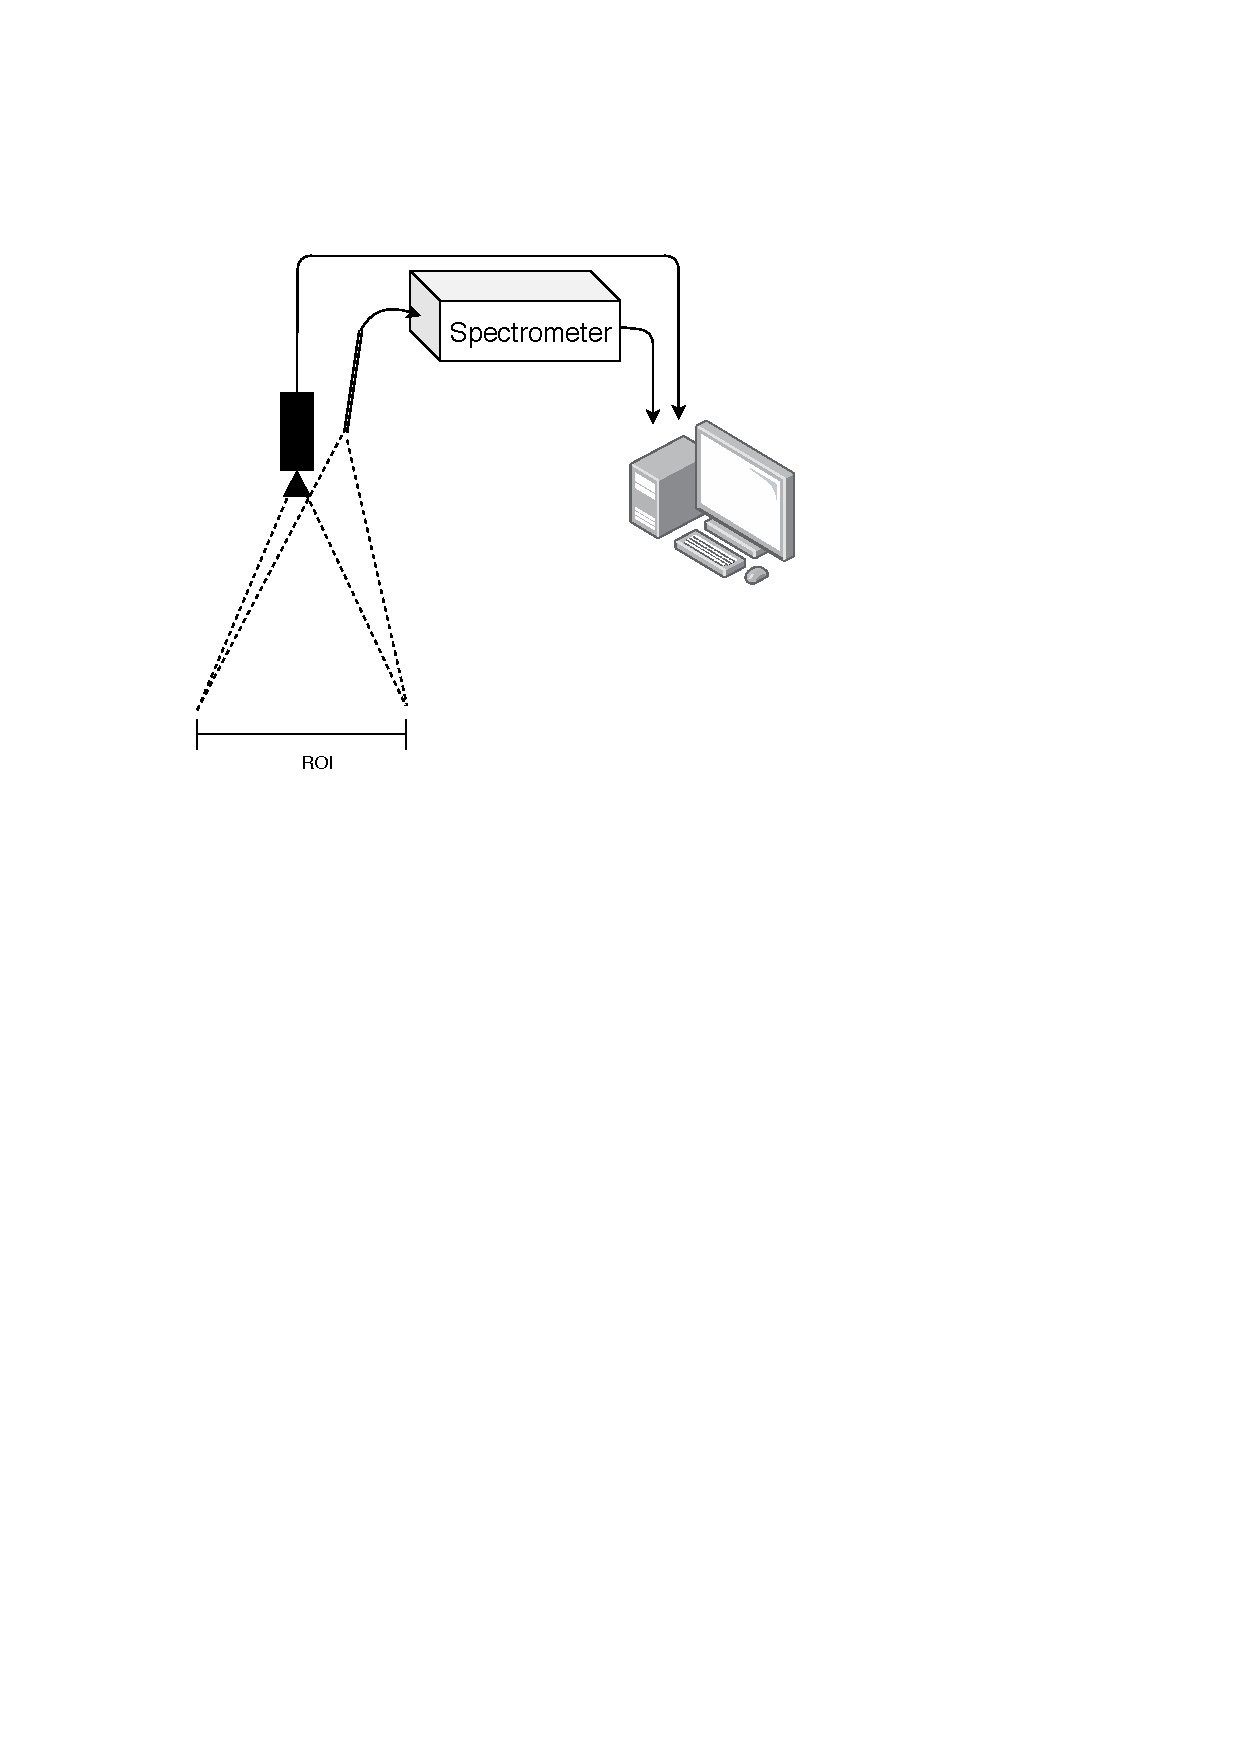
\includegraphics[]{figures/pt_setup.pdf}
    \caption{Setup}
    \label{}
\end{figure}


\section{Theory}



\section{Light}
Light is a crucial part of this project, as it is the source of input for both the camera and the spectrometer. It's also the link between the two sensors. The choosing of a sensor that can support both sensor types is therefore paramount. 

The characterization of the light source will be based on considerations from \cite{martinPracticalGuideMachine}, but also unfortunately be limited by available sources at the lab. This paper provides a longer checklist, that can be simplified greatly under the following conditions: Stationary objects, 




\bibliographystyle{unsrt}
\bibliography{references.bib}
\end{document}